\documentclass[12pt, titlepage]{article}

\usepackage{fullpage}
\usepackage[round]{natbib}
\usepackage{multirow}
\usepackage{booktabs}
\usepackage{tabularx}
\usepackage{graphicx}
\usepackage{float}
\usepackage{hyperref}
\hypersetup{
    colorlinks,
    citecolor=black,
    filecolor=black,
    linkcolor=red,
    urlcolor=blue
}
\usepackage[round]{natbib}

\newcounter{acnum}
\newcommand{\actheacnum}{AC\theacnum}
\newcommand{\acref}[1]{AC\ref{#1}}

\newcounter{ucnum}
\newcommand{\uctheucnum}{UC\theucnum}
\newcommand{\uref}[1]{UC\ref{#1}}

\newcounter{mnum}
\newcommand{\mthemnum}{M\themnum}
\newcommand{\mref}[1]{M\ref{#1}}

\title{SE 3XA3: Software Requirements Specification\\Title of Project}

\author{Team \#24, Node Messenger
		\\ Tasin Ahmed - ahmedm31
		\\ Shardool Patel - pates25
		\\ Omar Elemary - elemaryo
}

\date{\today}

\begin{document}

\maketitle

\pagenumbering{roman}
\tableofcontents
\listoftables
\listoffigures

\section{Major Revision History}
\begin{table}[h!]
\centering
\begin{tabular}{ccc}
\hline 
Revision & Date & Change \\ 
\hline 
Revision 0 & Date 1 & Notes \\ 
Revision 1 & Date 2 & Notes \\ 
\hline 
\end{tabular} 
\caption{Revision Control}
\label{my-label}
\end{table}

\pagenumbering{arabic}

\section{Introduction}
\subsection{Overview}
As the world becomes increasingly more connected through the internet, many common internet users are looking for an easy way to communicate with each other or reach out to distant loved ones. The market for messengers has become saturated with products that put the goal of earning maximum revenue over the needs of the consumer. Node Messenger's focus is to capture consumer interest by implementing a free and accessible web application messenger that allows them to personalize their experience and chat with other users in a simple, clean and non-intrusive way. Node messenger will become a haven for users searching for a consumer-friendly product with great functionality and cross-platform support.

\subsection{Context}
This document is the Module Guide (MG), created after the completion of the Software Requirements Specifications (SRS. The SRS lists the functional and non-functional requirements for the development of the project. The MG shows how the project meets the functional and non-functional requirements mentioned in the SRS, as well as showing how the modules are broken up in the project.

Following the creation of the MG, comes the creation of the Module Interface Specification (MIS). The MIS specifies the functions of each of the modules mentioned in the MG. It does so by documenting the variables, inputs, outputs, and exceptions for each module. 

\subsection{Design Principles}
There are two main we will be using for our project is Encapsulation and Abstraction. Encapsulation is when objects keep their states private, in a class. We will be using encapsulation in order to hide sensitive user information from being accessed by others. This can include the user's email, password, name, phone number etc. Abstraction will be used to make our messaging app more user friendly and eaasy to use. If the user has used other messaging apps prior to NodeM, they should have the necessary knowledge required to use our app already.

\subsection{Document Structure}
The rest of the document is organized as follows: 
\begin{itemize}
\item Section \ref{SecChange} lists the anticipated and unlikely changes of the software requirements.
\item Section \ref{SecMH} summarizes the module decomposition that was constructed according to the likely changes.
\item Section \ref{SecConnection} specifies the connections between the software requirements and the modules.
\item Section \ref{SecMD} gives a detailed description of the modules.
\item Section \ref{SecTM} includes two traceability matrices. One checks the completeness of the design against the requirements provided in the SRS. The other shows the relation between anticipated changes and the modules.
\item Section \ref{SecUse} describes the use relation between modules.
\end{itemize}

\section{Anticipated and Unlikely Changes} \label{SecChange}

\subsection{Anticipated Changes} \label{SecAchange}
\begin{description}
\item[\refstepcounter{acnum} \actheacnum \label{acColor}:] The color theme of the messaging app.
\item[\refstepcounter{acnum} \actheacnum \label{acMessage}:] The format of the message box.
\item[\refstepcounter{acnum} \actheacnum \label{acLogin}:] The format of the Login/Register screen.
\item[\refstepcounter{acnum} \actheacnum \label{acDomain}:] Domain name.
\item[\refstepcounter{acnum} \actheacnum \label{acButtons}:] Addition or removal of Buttons, and their functions.
\item[\refstepcounter{acnum} \actheacnum \label{acGUI}:] The Graphical User Interference for sending and receiving messages.
\item[\refstepcounter{acnum} \actheacnum \label{acSettings}:] The settings available to every user.
\end{description}

\subsection{Unlikely Changes} \label{SecUchange}
\begin{description}
\item[\refstepcounter{ucnum} \uctheucnum \label{ucIO}:] Input/Output devices.
\item[\refstepcounter{ucnum} \uctheucnum \label{ucIO}:] The programming languages.
\item[\refstepcounter{ucnum} \uctheucnum \label{ucIO}:] The format of React components.
\item[\refstepcounter{ucnum} \uctheucnum \label{ucIO}:] The goal of the project: send and receive messages from other users.
\end{description}

\section{Module Hierarchy} \label{SecMH}

This section provides an overview of the module design. Modules are summarized
in a hierarchy decomposed by secrets in Table \ref{TblMH}. The  modules listed
below in Table \ref{TblMHH}, which are leaves in the hierarchy tree, are the modules that will
actually be implemented.

\begin{table}[!htbp]
	\begin{tabular}{ll}
		\toprule
		Module Name & Module Number \\
		\midrule
		Hardware Hiding Module & M1\\
		\midrule
		Login Module \label{login} & M2\\
		\midrule
		Sign up Module \label{signup} & M3\\
		\midrule
		Sign in Module \label{sigin} & M4\\
		\midrule
		Chat Module \label{chat} & M5\\
		\midrule
		App Module \label{app} & M6\\
		\midrule
		Index Module \label{index} & M7\\
		\bottomrule
	\end{tabular}
	\caption{Module Number Format}
	\label{TblMHH}
\end{table}

\begin{table}[h!]
\centering
\begin{tabular}{p{0.3\textwidth} p{0.6\textwidth}}
\toprule
\textbf{Level 1} & \textbf{Level 2}\\
\midrule

{Hardware-Hiding Module} & ~ \\
\midrule

\multirow{7}{0.3\textwidth}{Behaviour-Hiding Module}\\
& Index Module\\
& Login Module\\
& Sign in Module\\
& Sign up Module\\
\midrule

\multirow{3}{0.3\textwidth}{Software Decision Module} & App Module\\
& Chat Module\\
\bottomrule

\end{tabular}
\caption{Module Hierarchy}
\label{TblMH}
\end{table}

\newpage

\section{Connection Between Requirements and Design} \label{SecConnection}

The design of the system is intended to satisfy the requirements developed in
the SRS. In this stage, the system is decomposed into modules. The connection
between requirements and modules is listed in Table \ref{TblRT}.

\section{Module Decomposition} \label{SecMD}

Modules are decomposed according to the principle of ``information hiding''
proposed by \citet{ParnasEtAl1984}. The \emph{Secrets} field in a module
decomposition is a brief statement of the design decision hidden by the
module. The \emph{Services} field specifies \emph{what} the module will do
without documenting \emph{how} to do it. For each module, a suggestion for the
implementing software is given under the \emph{Implemented By} title. If the
entry is \emph{OS}, this means that the module is provided by the operating
system or by standard programming language libraries.  Also indicate if the
module will be implemented specifically for the software.

Only the leaf modules in the
hierarchy have to be implemented. If a dash (\emph{--}) is shown, this means
that the module is not a leaf and will not have to be implemented. Whether or
not this module is implemented depends on the programming language
selected.

\subsection{Hardware Hiding Modules M1}

\begin{description}
\item[Secrets:]The data structure and algorithm used to implement the virtual
  hardware.
\item[Services:]Serves as a virtual hardware used by the rest of the
  system. This module provides the interface between the hardware and the
  software. So, the system can use it to display outputs or to accept inputs.
\item[Implemented By:] OS
\end{description}

\subsection{Behaviour-Hiding Module}

\begin{description}
\item[Secrets:]The contents of the required behaviours.
\item[Services:]Includes programs that provide externally visible behaviour of
  the system as specified in the software requirements specification (SRS)
  documents. This module serves as a communication layer between the
  hardware-hiding module and the software decision module. The programs in this
  module will need to change if there are changes in the SRS.
\item[Implemented By:] --
\end{description}

\subsubsection{Index Module M7}

\begin{description}
\item[Secrets:]Components used for web application.
\item[Services:]Generates API and element setup required to produce functioning web application.
\item[Implemented By:] React, HTML, JavaScript, CSS
\end{description}

\subsubsection{Sign in Module M4}
\begin{description}
\item[Secrets:]Sign in implementation.
\item[Services:]Describes and renders \textit{Sign in} logic and it's handles.
\item[Implemented By:] React, JavaScript
\end{description}

\subsubsection{Sign up Module M3}
\begin{description}
\item[Secrets:]Sign up implementation.
\item[Services:]Describes and renders \textit{Sign up} logic and it's handles.
\item[Implemented By:] React, JavaScript
\end{description}

\subsubsection{Login Module M2}
\begin{description}
\item[Secrets:]Sign in and Sign up implementation.
\item[Services:]Renders login web page utilizing \textit{Sign in} and \textit{Sign up} modules.
\item[Implemented By:] React, JavaScript, CSS
\end{description}



\subsection{Software Decision Module}

\begin{description}
\item[Secrets:] The design decision based on mathematical theorems, physical
  facts, or programming considerations. The secrets of this module are
  \emph{not} described in the SRS.
\item[Services:] Includes data structure and algorithms used in the system that
  do not provide direct interaction with the user. 
  % Changes in these modules are more likely to be motivated by a desire to
  % improve performance than by externally imposed changes.
\item[Implemented By:] --
\end{description}

\subsubsection{App Module M6}
\begin{description}
\item[Secrets:]Sign in, Sign up, Sign out authentication.
\item[Services:]Initializes and renders web app components while implementing their logic and handles.
\item[Implemented By:] React, JavaScript, CSS
\end{description}

\subsubsection{Chat Module M5}
\begin{description}
\item[Secrets:]Input, Output.
\item[Services:]Converts the input data into output messages sent by the user.
\item[Implemented By:] React, JavaScript, CSS
\end{description}

\section{Traceability Matrix} \label{SecTM}

This section shows two traceability matrices: between the modules and the
requirements and between the modules and the anticipated changes.

% the table should use mref, the requirements should be named, use something
% like fref
\begin{table}[H]
\centering
\begin{tabular}{p{0.2\textwidth} p{0.6\textwidth}}
\toprule
\textbf{Req.} & \textbf{Modules}\\
\midrule
R1 & M6, M7\\
R2 & M2, M4, M6\\
R3 & M2, M4, M6\\
R4 & M2, M4, M6\\
R5 & M2, M3, M6\\
R7 & M5\\
R14 & M5\\
R15 & M5\\
R18 & M5\\
\bottomrule
\end{tabular}
\caption{Trace Between Requirements and Modules}
\label{TblRT}
\end{table}

\textbf{NOTE: SOME REQUIREMENTS LISTED IN SRS DOCUMENT ARE NO LONGER IN THE SCOPE OF THE PROJECT AND WILL BE UPDATED IN REVISION 1}

\begin{table}[H]
\centering
\begin{tabular}{p{0.2\textwidth} p{0.6\textwidth}}
\toprule
\textbf{AC} & \textbf{Modules}\\
\midrule
\acref{acColor} & M2, M3, M4, M5, M6, M7\\
\acref{acMessage} & M5\\
\acref{acLogin} & M2\\
\acref{acDomain} & M7\\
\acref{acButtons} & M2, M3, M4\\
\acref{acGUI} & M5\\
\acref{acSettings} & M5\\
\bottomrule
\end{tabular}
\caption{Trace Between Anticipated Changes and Modules}
\label{TblACT}
\end{table}

\section{Use Hierarchy Between Modules} \label{SecUse}

In this section, the uses hierarchy between modules is
provided. \citet{Parnas1978} said of two programs A and B that A {\em uses} B if
correct execution of B may be necessary for A to complete the task described in
its specification. That is, A {\em uses} B if there exist situations in which
the correct functioning of A depends upon the availability of a correct
implementation of B.  Figure \ref{FigUH} illustrates the use relation between
the modules. It can be seen that the graph is a directed acyclic graph
(DAG). Each level of the hierarchy offers a testable and usable subset of the
system, and modules in the higher level of the hierarchy are essentially simpler
because they use modules from the lower levels.

\begin{figure}[H]
\centering
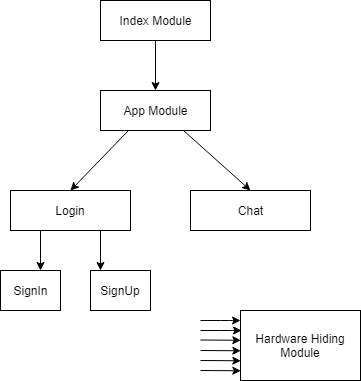
\includegraphics[width=0.5\textwidth]{usesHierarchy.png}
\caption{Use hierarchy among modules}
\label{FigUH}
\end{figure}

%\section*{References}

\bibliographystyle {plainnat}
\bibliography {MG}

\end{document}
